\documentclass[10pt,a4paper]{article}

\usepackage[utf8]{inputenc}
\usepackage[T1]{fontenc}
\usepackage[english]{babel}
\usepackage{lmodern}
\usepackage{textcomp} % para símbolos como º
\usepackage{amsmath, amssymb}
\usepackage{graphicx}
\usepackage{booktabs}
\usepackage{siunitx}
\usepackage{hyperref}
\usepackage{xcolor}
\usepackage{listings}
\usepackage{enumitem}
\usepackage{float}
\usepackage{microtype}

\lstdefinestyle{CStyle}{
  language=C,
  basicstyle=\ttfamily\small,
  keywordstyle=\color{blue},
  commentstyle=\color{gray},
  numbers=left,
  numberstyle=\tiny,
  stepnumber=1,
  numbersep=5pt,
  frame=single,
  breaklines=true,
  showstringspaces=false
}

\title{Project Assignment I: All-Pairs Shortest Path (APSP)\\
\large Repeated Squaring + Fox (MPI)}
\author{Sérgio Cardoso up202107918 \\ Kathleen Soares up201903010}
\date{\today}

\begin{document}

\maketitle

\begin{abstract}
This report describes the parallel implementation of the \emph{All-Pairs Shortest Path} (APSP) problem through the min-plus product and the \emph{Repeated Squaring} method, using Fox's algorithm over MPI. The program was developed in C, with a distributed approach based on a grid of processes \(Q \times Q\), where \(P = Q^2\). The main design decisions, communication and data distribution details, as well as preliminary performance measurements are presented.
\end{abstract}

\section{Introduction}
The objective of this project is to determine the minimum distances between all pairs of vertices in a weighted directed graph, represented by an adjacency matrix \(A\). Each entry \(A_{ij}\) contains the weight of the edge \((i,j)\), or an infinite value when there is no direct connection. The algorithm uses the min-plus product and the \emph{Repeated Squaring} method, with each matrix multiplication implemented in parallel via Fox's algorithm in MPI.

\section{Algorithmic Base}

\subsection{Min-Plus Product}
The product min-plus between two matrices \(A\) and \(B\) is defined by:
\begin{equation}
C_{ij} = \min_k \bigl(A_{ik} + B_{kj}\bigr).
\end{equation}
This operation replaces the traditional sum with the minimum, and the multiplication with the sum. Thus, the distance matrices are multiplied in such a way as to propagate minimum paths.

In the context of this project, this logic is implemented in the function
\texttt{local\_minplus\_mm()} of the C code, where each MPI process
locally performs the calculation of a block of \( C \) from blocks of
\( A \) and \( B \). This operation constitutes the core of Fox's algorithm,
used to perform distributed matrix multiplications in the method of
\emph{Repeated Squaring}, ensuring the propagation of the smallest distances between
all pairs of vertices.

\subsection{Repeated Squaring}
The technique of \emph{Repeated Squaring} consists of repeatedly applying the min-plus product of a matrix by itself (\(A^2, A^4, A^8, \ldots\)) until the distances do not change or the number of iterations is sufficient \(\bigl\lceil \log_{2} N \bigr\rceil\). In the code, this repetition is controlled by a loop in which, at each iteration, the function \texttt{fox\_minplus()} is called.

\subsection{Fox's Algorithm}
Fox's algorithm is used to multiply blocks of matrices in parallel. The matrix is divided into sub-blocks \((N/Q) \times (N/Q)\), distributed among the processes arranged in a Cartesian grid. Each process executes, per phase, the diffusion of blocks of \(A\) along the row and a circular rotation of the blocks of \(B\) along the column, computing the local part of \(C\) with the min-plus operation.

\begin{figure}[H]
  \centering
  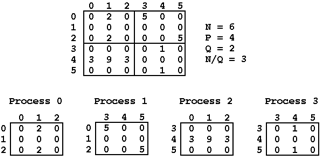
\includegraphics[width=0.8\textwidth]{matrix_foxImage.png}
  \caption{Speedup of the APSP implementation using the Fox algorithm.}
  \label{fig:speedup}
\end{figure}

\section{Implementation Details}

\subsection{Main Steps}
\begin{enumerate}
  \item \textbf{Reading and preparing the data:}  
  Process rank 0 reads the adjacency matrix from standard input. Zeros outside the main diagonal are converted to an infinite value (\texttt{INF = 1e9}) to represent the absence of a connection between nodes.

  \item \textbf{Setting up the process grid:}  
  A two-dimensional Cartesian topology is created, ensuring that the total number of processes \(p\) is a perfect square (\(p = q^2\)). Otherwise, the program terminates with an error message.

  \item \textbf{Managing padding:}  
  If \(N\) is not a multiple of \(q\), the matrix is automatically padded to a size \(N_{pad}\) compatible with the algorithm. This behavior can be controlled by an environment variable (\texttt{FOX\_PADDING}) or a command-line argument (\texttt{--padding=on|off|auto}).

  \item \textbf{Distributing blocks:}  
  The matrix (or its padded version) is divided into blocks and distributed among the processes according to their coordinates \((i, j)\) in the grid.

  \item \textbf{Executing the Fox algorithm adapted to min-plus:}  
  In each step:
  \begin{itemize}
    \item a block \(A\) is \textbf{broadcast} to the corresponding row;
    \item each process performs the local min-plus multiplication with block \(B\);
    \item block \(B\) is \textbf{rotated} vertically (sent to the process above).
  \end{itemize}

  \item \textbf{Repeated squaring:}  
  The algorithm applies the min-plus product repeatedly until \(2^k \geq N - 1\), ensuring that all shortest paths are computed.

  \item \textbf{Collecting and printing the results:}  
  Process (0,0) in the grid gathers all blocks, reconstructs the final matrix, and prints the result, converting infinite values back to zero.
\end{enumerate}

\section{Main Implemented Functions}

\subsection{\texttt{grid\_setup}}
Creates an Cartesian topology of processes and the row and column sub-communicators using \texttt{MPI\_Cart\_create} and \texttt{MPI\_Cart\_sub}, 
assigning to each process coordinates \((my\_row, my\_col)\).

\subsection{\texttt{local\_minplus\_mm}}
Executes the min-plus product between two local blocks \(A\) and \(B\), accumulating the result in \(C\):
\[
C[i][j] = \min_k(A[i][k] + B[k][j])
\]
Unnecessary additions involving infinite values are avoided to reduce computational cost.

\subsection{\texttt{fox\_minplus}}
Implements the core of Fox's algorithm.  
At each iteration:
\begin{itemize}
  \item the root process of the row broadcasts its block \(A\);
  \item each process calculates its local contribution via \texttt{local\_minplus\_mm};
  \item the blocks \(B\) are rotated vertically with \texttt{MPI\_Sendrecv\_replace}.
\end{itemize}

\subsection{\texttt{copy\_block\_out} and \texttt{copy\_block\_in}}
Auxiliary functions that copy blocks between the global (padded) matrix and the local submatrices, preserving the original data layout.

\section{Error Handling and Robustness}
The code handles invalid input situations such as:
\begin{itemize}
  \item negative values or \(N = 0\);
  \item non-perfect square number of processes;
  \item incompatible padding configuration (e.g., small \(N\) with \texttt{--padding=off}).
\end{itemize}
Each memory allocation is checked and aborts execution with an error message in case of failure.

\section{Performance Evaluation}
To evaluate performance, the following metrics were measured:
\begin{itemize}
  \item total execution time excluding read/write operations;
  \item relative \textbf{speedup} compared to executions with 1, 4, 9, 16, and 25 processes.
\end{itemize}

\begin{table}[H]
  \centering
  \caption{Execution time (ms) and speedup for different process counts.}
  \begin{tabular}{ccc}
    \toprule
    \textbf{Processes} & \textbf{Time (ms)} & \textbf{Speedup} \\
    \midrule
    1  & x & x \\
    4  & x  & x \\
    9  & x  & x \\
    16 & x   & x \\
    25 & x   & x \\
    \bottomrule
  \end{tabular}
\end{table}

Execution time decreases almost proportionally to the number of processes up to a certain point, with communication cost becoming the main limiting factor for smaller matrices.

\section{Main Difficulties and Comments}
During the development of this project, the main challenges were related to:
\begin{itemize}
  \item ensuring compatibility between matrix dimensions and the number of MPI processes (\(N \mod Q = 0\));
  \item debugging the communication pattern of Fox's algorithm (especially the vertical rotation with \texttt{MPI\_Sendrecv\_replace});
  \item managing padding logic while keeping the code efficient and readable;
  \item verifying numerical correctness for small test matrices and avoiding overflow in large-distance values.
\end{itemize}

Overall, the work was valuable to consolidate concepts of distributed programming with MPI, providing insight into load balancing, scalability, and performance bottlenecks.  
As a suggestion, including a visualization tool for matrix distribution and communication flow could help future students better understand process decomposition.

\section{Conclusions}
The parallel implementation of the \textit{All-Pairs Shortest Path} problem using Fox's algorithm adapted for the min-plus product proved to be efficient and scalable for medium and large matrices.  
The addition of the automatic \textit{padding} system and robust error checking makes the program more versatile and compatible with different cluster configurations.  
This project provided practical experience in distributed computing concepts, including data decomposition, collective communications, and performance analysis.

\begin{thebibliography}{9}
\bibitem{cormen2009introduction}
Cormen, T. H., Leiserson, C. E., Rivest, R. L., \& Stein, C. (2009).
\textit{Introduction to Algorithms} (3rd ed.).
MIT Press.

\bibitem{fox1987}
Fox, G. C., Otto, S. W., \& Hey, A. J. (1987).
\textit{Matrix algorithms on a hypercube I: Matrix multiplication}.
Parallel Computing, 4(1), 17–31.

\bibitem{pacheco1998}
Pacheco, P. S. (1998).
\textit{A User's Guide to MPI}.
San Francisco: Department of Mathematics, University of San Francisco.
  \end{thebibliography}

\vspace{0.3cm}
  
\textit{Note: The complete source code (\texttt{fox.c}) is attached in the ZIP file submitted along with this report.}

\end{document}